\documentclass[twoside]{book}

% Packages required by doxygen
\usepackage{fixltx2e}
\usepackage{calc}
\usepackage{doxygen}
\usepackage[export]{adjustbox} % also loads graphicx
\usepackage{graphicx}
\usepackage[utf8]{inputenc}
\usepackage{makeidx}
\usepackage{multicol}
\usepackage{multirow}
\PassOptionsToPackage{warn}{textcomp}
\usepackage{textcomp}
\usepackage[nointegrals]{wasysym}
\usepackage[table]{xcolor}

% Font selection
\usepackage[T1]{fontenc}
\usepackage[scaled=.90]{helvet}
\usepackage{courier}
\usepackage{amssymb}
\usepackage{sectsty}
\renewcommand{\familydefault}{\sfdefault}
\allsectionsfont{%
  \fontseries{bc}\selectfont%
  \color{darkgray}%
}
\renewcommand{\DoxyLabelFont}{%
  \fontseries{bc}\selectfont%
  \color{darkgray}%
}
\newcommand{\+}{\discretionary{\mbox{\scriptsize$\hookleftarrow$}}{}{}}

% Page & text layout
\usepackage{geometry}
\geometry{%
  a4paper,%
  top=2.5cm,%
  bottom=2.5cm,%
  left=2.5cm,%
  right=2.5cm%
}
\tolerance=750
\hfuzz=15pt
\hbadness=750
\setlength{\emergencystretch}{15pt}
\setlength{\parindent}{0cm}
\setlength{\parskip}{3ex plus 2ex minus 2ex}
\makeatletter
\renewcommand{\paragraph}{%
  \@startsection{paragraph}{4}{0ex}{-1.0ex}{1.0ex}{%
    \normalfont\normalsize\bfseries\SS@parafont%
  }%
}
\renewcommand{\subparagraph}{%
  \@startsection{subparagraph}{5}{0ex}{-1.0ex}{1.0ex}{%
    \normalfont\normalsize\bfseries\SS@subparafont%
  }%
}
\makeatother

% Headers & footers
\usepackage{fancyhdr}
\pagestyle{fancyplain}
\fancyhead[LE]{\fancyplain{}{\bfseries\thepage}}
\fancyhead[CE]{\fancyplain{}{}}
\fancyhead[RE]{\fancyplain{}{\bfseries\leftmark}}
\fancyhead[LO]{\fancyplain{}{\bfseries\rightmark}}
\fancyhead[CO]{\fancyplain{}{}}
\fancyhead[RO]{\fancyplain{}{\bfseries\thepage}}
\fancyfoot[LE]{\fancyplain{}{}}
\fancyfoot[CE]{\fancyplain{}{}}
\fancyfoot[RE]{\fancyplain{}{\bfseries\scriptsize Generated by Doxygen }}
\fancyfoot[LO]{\fancyplain{}{\bfseries\scriptsize Generated by Doxygen }}
\fancyfoot[CO]{\fancyplain{}{}}
\fancyfoot[RO]{\fancyplain{}{}}
\renewcommand{\footrulewidth}{0.4pt}
\renewcommand{\chaptermark}[1]{%
  \markboth{#1}{}%
}
\renewcommand{\sectionmark}[1]{%
  \markright{\thesection\ #1}%
}

% Indices & bibliography
\usepackage{natbib}
\usepackage[titles]{tocloft}
\setcounter{tocdepth}{3}
\setcounter{secnumdepth}{5}
\makeindex

% Custom commands
\newcommand{\clearemptydoublepage}{%
  \newpage{\pagestyle{empty}\cleardoublepage}%
}

\usepackage{caption}
\captionsetup{labelsep=space,justification=centering,font={bf},singlelinecheck=off,skip=4pt,position=top}

%===== C O N T E N T S =====

\begin{document}

% Titlepage & ToC
\pagenumbering{alph}
\begin{titlepage}
\vspace*{7cm}
\begin{center}%
{\Large Projeto2 \\[1ex]\large 1.\+0 }\\
\vspace*{1cm}
{\large Generated by Doxygen 1.8.14}\\
\end{center}
\end{titlepage}
\clearemptydoublepage
\pagenumbering{roman}
\tableofcontents
\clearemptydoublepage
\pagenumbering{arabic}

%--- Begin generated contents ---
\chapter{Hierarchical Index}
\section{Class Hierarchy}
This inheritance list is sorted roughly, but not completely, alphabetically\+:\begin{DoxyCompactList}
\item \contentsline{section}{Figura\+Geometrica}{\pageref{class_figura_geometrica}}{}
\begin{DoxyCompactList}
\item \contentsline{section}{Circulo}{\pageref{class_circulo}}{}
\item \contentsline{section}{Retangulo}{\pageref{class_retangulo}}{}
\end{DoxyCompactList}
\item \contentsline{section}{Reta}{\pageref{class_reta}}{}
\item \contentsline{section}{Screen}{\pageref{class_screen}}{}
\end{DoxyCompactList}

\chapter{Class Index}
\section{Class List}
Here are the classes, structs, unions and interfaces with brief descriptions\+:\begin{DoxyCompactList}
\item\contentsline{section}{\textbf{ Circulo} }{\pageref{class_circulo}}{}
\item\contentsline{section}{\textbf{ Figura\+Geometrica} }{\pageref{class_figura_geometrica}}{}
\item\contentsline{section}{\textbf{ Reta} }{\pageref{class_reta}}{}
\item\contentsline{section}{\textbf{ Retangulo} }{\pageref{class_retangulo}}{}
\item\contentsline{section}{\textbf{ Screen} }{\pageref{class_screen}}{}
\end{DoxyCompactList}

\chapter{File Index}
\section{File List}
Here is a list of all files with brief descriptions\+:\begin{DoxyCompactList}
\item\contentsline{section}{C\+:/\+Users/\+Adamstor Pequeno/\+Desktop/jooj/\textbf{ circulo.\+cpp} }{\pageref{circulo_8cpp}}{}
\item\contentsline{section}{C\+:/\+Users/\+Adamstor Pequeno/\+Desktop/jooj/\textbf{ circulo.\+h} }{\pageref{circulo_8h}}{}
\item\contentsline{section}{C\+:/\+Users/\+Adamstor Pequeno/\+Desktop/jooj/\textbf{ figurageometrica.\+cpp} }{\pageref{figurageometrica_8cpp}}{}
\item\contentsline{section}{C\+:/\+Users/\+Adamstor Pequeno/\+Desktop/jooj/\textbf{ figurageometrica.\+h} }{\pageref{figurageometrica_8h}}{}
\item\contentsline{section}{C\+:/\+Users/\+Adamstor Pequeno/\+Desktop/jooj/\textbf{ main.\+cpp} }{\pageref{main_8cpp}}{}
\item\contentsline{section}{C\+:/\+Users/\+Adamstor Pequeno/\+Desktop/jooj/\textbf{ reta.\+cpp} }{\pageref{reta_8cpp}}{}
\item\contentsline{section}{C\+:/\+Users/\+Adamstor Pequeno/\+Desktop/jooj/\textbf{ reta.\+h} }{\pageref{reta_8h}}{}
\item\contentsline{section}{C\+:/\+Users/\+Adamstor Pequeno/\+Desktop/jooj/\textbf{ retangulo.\+cpp} }{\pageref{retangulo_8cpp}}{}
\item\contentsline{section}{C\+:/\+Users/\+Adamstor Pequeno/\+Desktop/jooj/\textbf{ retangulo.\+h} }{\pageref{retangulo_8h}}{}
\item\contentsline{section}{C\+:/\+Users/\+Adamstor Pequeno/\+Desktop/jooj/\textbf{ screen.\+cpp} }{\pageref{screen_8cpp}}{}
\item\contentsline{section}{C\+:/\+Users/\+Adamstor Pequeno/\+Desktop/jooj/\textbf{ screen.\+h} }{\pageref{screen_8h}}{}
\end{DoxyCompactList}

\chapter{Class Documentation}
\section{Circulo Class Reference}
\label{class_circulo}\index{Circulo@{Circulo}}


{\ttfamily \#include $<$circulo.\+h$>$}

Inheritance diagram for Circulo\+:\begin{figure}[H]
\begin{center}
\leavevmode
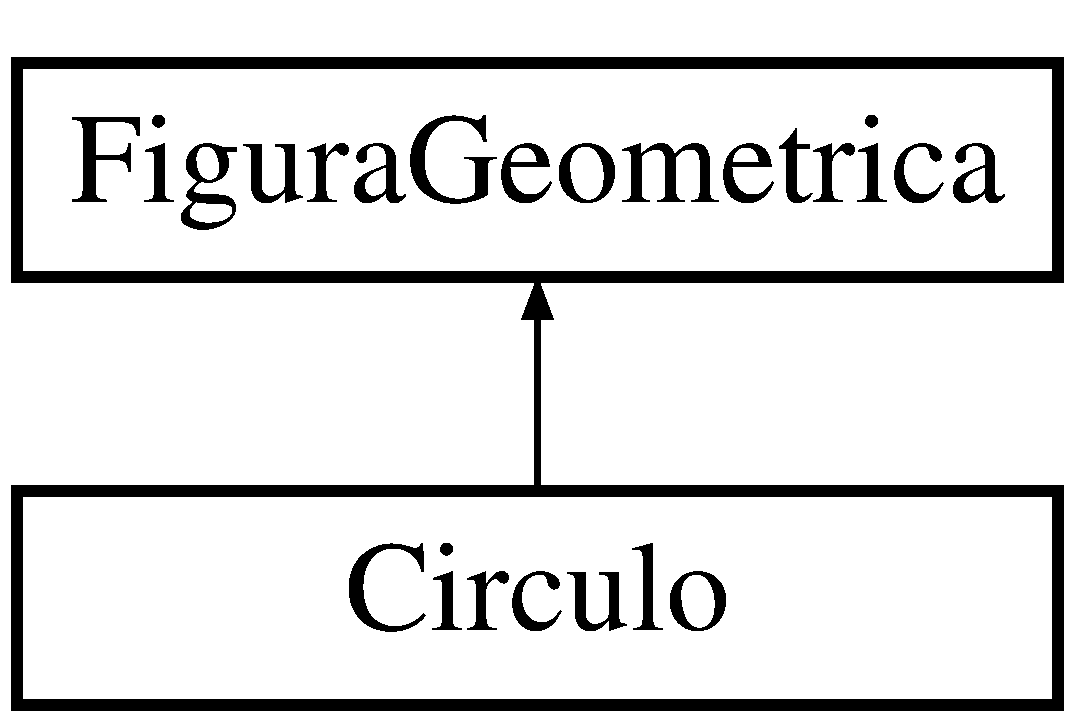
\includegraphics[height=2.000000cm]{class_circulo}
\end{center}
\end{figure}
\subsection*{Public Member Functions}
\begin{DoxyCompactItemize}
\item 
\textbf{ Circulo} ()
\item 
void \textbf{ draw} ()
\begin{DoxyCompactList}\small\item\em função virtual para desenho de figuras geometricas \end{DoxyCompactList}\end{DoxyCompactItemize}


\subsection{Constructor \& Destructor Documentation}
\mbox{\label{class_circulo_a6933bf908b78a4167684081a3a8f257f}} 
\index{Circulo@{Circulo}!Circulo@{Circulo}}
\index{Circulo@{Circulo}!Circulo@{Circulo}}
\subsubsection{Circulo()}
{\footnotesize\ttfamily Circulo\+::\+Circulo (\begin{DoxyParamCaption}{ }\end{DoxyParamCaption})}



\subsection{Member Function Documentation}
\mbox{\label{class_circulo_aa94899872fb6c586d1343df1d9ce0d86}} 
\index{Circulo@{Circulo}!draw@{draw}}
\index{draw@{draw}!Circulo@{Circulo}}
\subsubsection{draw()}
{\footnotesize\ttfamily void Circulo\+::draw (\begin{DoxyParamCaption}{ }\end{DoxyParamCaption})\hspace{0.3cm}{\ttfamily [virtual]}}



função virtual para desenho de figuras geometricas 



Implements \textbf{ Figura\+Geometrica} \doxyref{}{p.}{class_figura_geometrica_ad71f2e6286d1e5e4dce76a3e5533c6ff}.



The documentation for this class was generated from the following files\+:\begin{DoxyCompactItemize}
\item 
C\+:/\+Users/\+Adamstor Pequeno/\+Desktop/jooj/\textbf{ circulo.\+h}\item 
C\+:/\+Users/\+Adamstor Pequeno/\+Desktop/jooj/\textbf{ circulo.\+cpp}\end{DoxyCompactItemize}

\section{Figura\+Geometrica Class Reference}
\label{class_figura_geometrica}\index{Figura\+Geometrica@{Figura\+Geometrica}}


{\ttfamily \#include $<$figurageometrica.\+h$>$}

Inheritance diagram for Figura\+Geometrica\+:\begin{figure}[H]
\begin{center}
\leavevmode
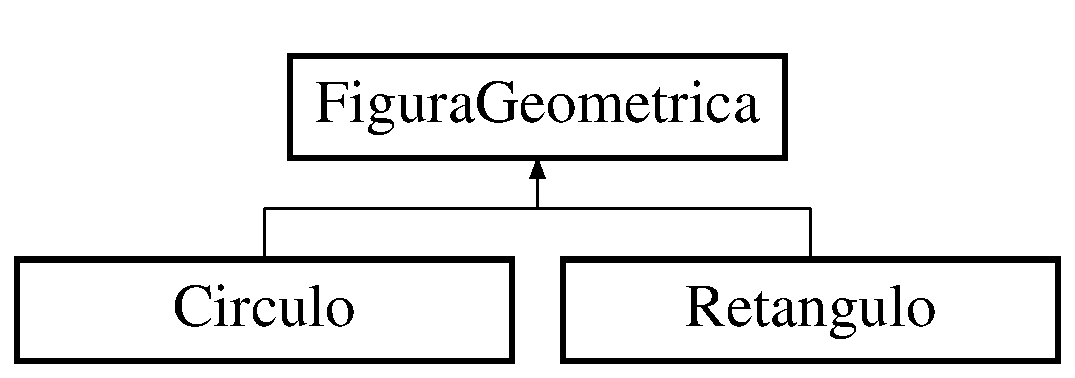
\includegraphics[height=2.000000cm]{class_figura_geometrica}
\end{center}
\end{figure}
\subsection*{Public Member Functions}
\begin{DoxyCompactItemize}
\item 
\textbf{ Figura\+Geometrica} ()
\begin{DoxyCompactList}\small\item\em Construtor padrão de uma figura geometrica. \end{DoxyCompactList}\item 
virtual void \textbf{ draw} ()=0
\begin{DoxyCompactList}\small\item\em função virtual para desenho de figuras geometricas \end{DoxyCompactList}\end{DoxyCompactItemize}


\subsection{Constructor \& Destructor Documentation}
\mbox{\label{class_figura_geometrica_a81d7c7efaea511e60a15f5a363138dd9}} 
\index{Figura\+Geometrica@{Figura\+Geometrica}!Figura\+Geometrica@{Figura\+Geometrica}}
\index{Figura\+Geometrica@{Figura\+Geometrica}!Figura\+Geometrica@{Figura\+Geometrica}}
\subsubsection{Figura\+Geometrica()}
{\footnotesize\ttfamily Figura\+Geometrica\+::\+Figura\+Geometrica (\begin{DoxyParamCaption}{ }\end{DoxyParamCaption})}



Construtor padrão de uma figura geometrica. 



\subsection{Member Function Documentation}
\mbox{\label{class_figura_geometrica_ad71f2e6286d1e5e4dce76a3e5533c6ff}} 
\index{Figura\+Geometrica@{Figura\+Geometrica}!draw@{draw}}
\index{draw@{draw}!Figura\+Geometrica@{Figura\+Geometrica}}
\subsubsection{draw()}
{\footnotesize\ttfamily void Figura\+Geometrica\+::draw (\begin{DoxyParamCaption}{ }\end{DoxyParamCaption})\hspace{0.3cm}{\ttfamily [pure virtual]}}



função virtual para desenho de figuras geometricas 



Implemented in \textbf{ Retangulo} \doxyref{}{p.}{class_retangulo_a48cb75fe7cd048727879c25485976444}, and \textbf{ Circulo} \doxyref{}{p.}{class_circulo_aa94899872fb6c586d1343df1d9ce0d86}.



The documentation for this class was generated from the following files\+:\begin{DoxyCompactItemize}
\item 
C\+:/\+Users/\+Adamstor Pequeno/\+Desktop/jooj/\textbf{ figurageometrica.\+h}\item 
C\+:/\+Users/\+Adamstor Pequeno/\+Desktop/jooj/\textbf{ figurageometrica.\+cpp}\end{DoxyCompactItemize}

\section{Reta Class Reference}
\label{class_reta}\index{Reta@{Reta}}


{\ttfamily \#include $<$reta.\+h$>$}

\subsection*{Public Member Functions}
\begin{DoxyCompactItemize}
\item 
\textbf{ Reta} (int \+\_\+x1, int \+\_\+y1, int \+\_\+x2, int \+\_\+y2)
\begin{DoxyCompactList}\small\item\em Construtor com argumentos para \doxyref{Reta}{p.}{class_reta} Recebe os pontos x,y iniciais primeiro e depois os pontos x,y finais para a reta. \end{DoxyCompactList}\item 
void \textbf{ draw} (\textbf{ Screen} \&s)
\begin{DoxyCompactList}\small\item\em Fun��o de desenho da \doxyref{Reta}{p.}{class_reta} usando os dados da reta, desenha ela numa matriz. \end{DoxyCompactList}\end{DoxyCompactItemize}


\subsection{Constructor \& Destructor Documentation}
\mbox{\label{class_reta_a156d293ea4e42a003eb5f8e55a67bf68}} 
\index{Reta@{Reta}!Reta@{Reta}}
\index{Reta@{Reta}!Reta@{Reta}}
\subsubsection{Reta()}
{\footnotesize\ttfamily Reta\+::\+Reta (\begin{DoxyParamCaption}\item[{int}]{\+\_\+x1,  }\item[{int}]{\+\_\+y1,  }\item[{int}]{\+\_\+x2,  }\item[{int}]{\+\_\+y2 }\end{DoxyParamCaption})}



Construtor com argumentos para \doxyref{Reta}{p.}{class_reta} Recebe os pontos x,y iniciais primeiro e depois os pontos x,y finais para a reta. 



\subsection{Member Function Documentation}
\mbox{\label{class_reta_a15a59889776093ceae4f3b13d42ffbd0}} 
\index{Reta@{Reta}!draw@{draw}}
\index{draw@{draw}!Reta@{Reta}}
\subsubsection{draw()}
{\footnotesize\ttfamily void Reta\+::draw (\begin{DoxyParamCaption}\item[{\textbf{ Screen} \&}]{s }\end{DoxyParamCaption})}



Fun��o de desenho da \doxyref{Reta}{p.}{class_reta} usando os dados da reta, desenha ela numa matriz. 



The documentation for this class was generated from the following files\+:\begin{DoxyCompactItemize}
\item 
C\+:/\+Users/\+Adamstor Pequeno/\+Desktop/jooj/\textbf{ reta.\+h}\item 
C\+:/\+Users/\+Adamstor Pequeno/\+Desktop/jooj/\textbf{ reta.\+cpp}\end{DoxyCompactItemize}

\section{Retangulo Class Reference}
\label{class_retangulo}\index{Retangulo@{Retangulo}}


{\ttfamily \#include $<$retangulo.\+h$>$}

Inheritance diagram for Retangulo\+:\begin{figure}[H]
\begin{center}
\leavevmode
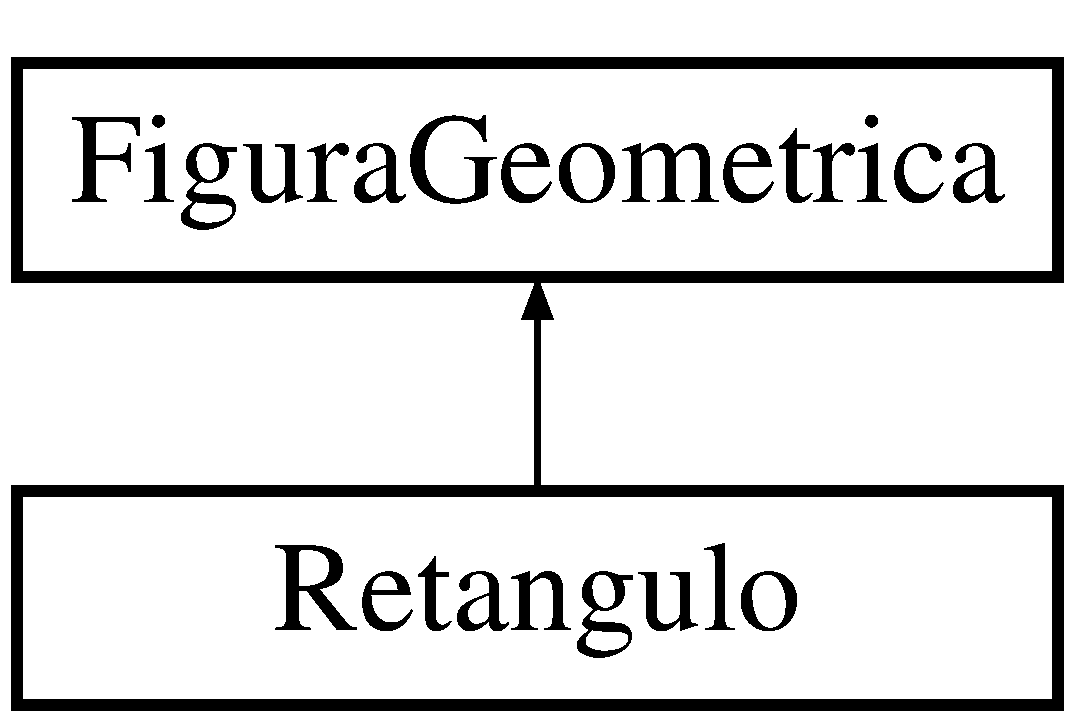
\includegraphics[height=2.000000cm]{class_retangulo}
\end{center}
\end{figure}
\subsection*{Public Member Functions}
\begin{DoxyCompactItemize}
\item 
\textbf{ Retangulo} ()
\begin{DoxyCompactList}\small\item\em construtor padrão de retângulo \end{DoxyCompactList}\item 
\textbf{ Retangulo} (int \+\_\+x0, int \+\_\+y0, int \+\_\+L, int \+\_\+H, bool \+\_\+fillmode)
\begin{DoxyCompactList}\small\item\em Construtor com argumentos do retângulo recebe os valores x,y do ponto inicial do retângulo, em seguida recebe sua largura, altura e uma variável de verdadeiro ou falso para ser preenchido ou não. \end{DoxyCompactList}\item 
void \textbf{ draw} ()
\begin{DoxyCompactList}\small\item\em Método para desenho do retângulo em uma matriz. \end{DoxyCompactList}\end{DoxyCompactItemize}


\subsection{Constructor \& Destructor Documentation}
\mbox{\label{class_retangulo_ac21a81cae046920c8bee401bcb879562}} 
\index{Retangulo@{Retangulo}!Retangulo@{Retangulo}}
\index{Retangulo@{Retangulo}!Retangulo@{Retangulo}}
\subsubsection{Retangulo()\hspace{0.1cm}{\footnotesize\ttfamily [1/2]}}
{\footnotesize\ttfamily Retangulo\+::\+Retangulo (\begin{DoxyParamCaption}{ }\end{DoxyParamCaption})}



construtor padrão de retângulo 

\mbox{\label{class_retangulo_a35f18f8491de3b475c27d88f6f351fb3}} 
\index{Retangulo@{Retangulo}!Retangulo@{Retangulo}}
\index{Retangulo@{Retangulo}!Retangulo@{Retangulo}}
\subsubsection{Retangulo()\hspace{0.1cm}{\footnotesize\ttfamily [2/2]}}
{\footnotesize\ttfamily Retangulo\+::\+Retangulo (\begin{DoxyParamCaption}\item[{int}]{\+\_\+x0,  }\item[{int}]{\+\_\+y0,  }\item[{int}]{\+\_\+L,  }\item[{int}]{\+\_\+H,  }\item[{bool}]{\+\_\+fillmode }\end{DoxyParamCaption})}



Construtor com argumentos do retângulo recebe os valores x,y do ponto inicial do retângulo, em seguida recebe sua largura, altura e uma variável de verdadeiro ou falso para ser preenchido ou não. 



\subsection{Member Function Documentation}
\mbox{\label{class_retangulo_a48cb75fe7cd048727879c25485976444}} 
\index{Retangulo@{Retangulo}!draw@{draw}}
\index{draw@{draw}!Retangulo@{Retangulo}}
\subsubsection{draw()}
{\footnotesize\ttfamily void Retangulo\+::draw (\begin{DoxyParamCaption}{ }\end{DoxyParamCaption})\hspace{0.3cm}{\ttfamily [virtual]}}



Método para desenho do retângulo em uma matriz. 

Desenha o retângulo numa matriz usando os valores dados anteriormente. 

Implements \textbf{ Figura\+Geometrica} \doxyref{}{p.}{class_figura_geometrica_ad71f2e6286d1e5e4dce76a3e5533c6ff}.



The documentation for this class was generated from the following files\+:\begin{DoxyCompactItemize}
\item 
C\+:/\+Users/\+Adamstor Pequeno/\+Desktop/jooj/\textbf{ retangulo.\+h}\item 
C\+:/\+Users/\+Adamstor Pequeno/\+Desktop/jooj/\textbf{ retangulo.\+cpp}\end{DoxyCompactItemize}

\section{Screen Class Reference}
\label{class_screen}\index{Screen@{Screen}}


{\ttfamily \#include $<$screen.\+h$>$}

\subsection*{Public Member Functions}
\begin{DoxyCompactItemize}
\item 
\textbf{ Screen} (int nlin, int ncol)
\item 
void \textbf{ set\+Pixel} (int x, int y)
\item 
void \textbf{ clear} ()
\item 
void \textbf{ set\+Brush} (char brush)
\end{DoxyCompactItemize}
\subsection*{Friends}
\begin{DoxyCompactItemize}
\item 
ostream \& \textbf{ operator$<$$<$} (ostream \&os, \textbf{ Screen} \&t)
\end{DoxyCompactItemize}


\subsection{Constructor \& Destructor Documentation}
\mbox{\label{class_screen_a246eac542489ef06335800fae60827ee}} 
\index{Screen@{Screen}!Screen@{Screen}}
\index{Screen@{Screen}!Screen@{Screen}}
\subsubsection{Screen()}
{\footnotesize\ttfamily Screen\+::\+Screen (\begin{DoxyParamCaption}\item[{int}]{nlin,  }\item[{int}]{ncol }\end{DoxyParamCaption})}



\subsection{Member Function Documentation}
\mbox{\label{class_screen_a35e74266b2a04e37b354ceff7a5f1031}} 
\index{Screen@{Screen}!clear@{clear}}
\index{clear@{clear}!Screen@{Screen}}
\subsubsection{clear()}
{\footnotesize\ttfamily void Screen\+::clear (\begin{DoxyParamCaption}{ }\end{DoxyParamCaption})}

\mbox{\label{class_screen_a14a00e158f99df199772172554a20576}} 
\index{Screen@{Screen}!set\+Brush@{set\+Brush}}
\index{set\+Brush@{set\+Brush}!Screen@{Screen}}
\subsubsection{set\+Brush()}
{\footnotesize\ttfamily void Screen\+::set\+Brush (\begin{DoxyParamCaption}\item[{char}]{brush }\end{DoxyParamCaption})}

\mbox{\label{class_screen_ae6bea81c57a22d226507c3c26fa95ee0}} 
\index{Screen@{Screen}!set\+Pixel@{set\+Pixel}}
\index{set\+Pixel@{set\+Pixel}!Screen@{Screen}}
\subsubsection{set\+Pixel()}
{\footnotesize\ttfamily void Screen\+::set\+Pixel (\begin{DoxyParamCaption}\item[{int}]{x,  }\item[{int}]{y }\end{DoxyParamCaption})}



\subsection{Friends And Related Function Documentation}
\mbox{\label{class_screen_aab6a2880746bfe1b7964817cc8f0989e}} 
\index{Screen@{Screen}!operator$<$$<$@{operator$<$$<$}}
\index{operator$<$$<$@{operator$<$$<$}!Screen@{Screen}}
\subsubsection{operator$<$$<$}
{\footnotesize\ttfamily ostream\& operator$<$$<$ (\begin{DoxyParamCaption}\item[{ostream \&}]{os,  }\item[{\textbf{ Screen} \&}]{t }\end{DoxyParamCaption})\hspace{0.3cm}{\ttfamily [friend]}}



The documentation for this class was generated from the following files\+:\begin{DoxyCompactItemize}
\item 
C\+:/\+Users/\+Adamstor Pequeno/\+Desktop/jooj/\textbf{ screen.\+h}\item 
C\+:/\+Users/\+Adamstor Pequeno/\+Desktop/jooj/\textbf{ screen.\+cpp}\end{DoxyCompactItemize}

\chapter{File Documentation}
\section{C\+:/\+Users/\+Adamstor Pequeno/\+Desktop/jooj/circulo.cpp File Reference}
\label{circulo_8cpp}\index{C\+:/\+Users/\+Adamstor Pequeno/\+Desktop/jooj/circulo.\+cpp@{C\+:/\+Users/\+Adamstor Pequeno/\+Desktop/jooj/circulo.\+cpp}}
{\ttfamily \#include \char`\"{}circulo.\+h\char`\"{}}\newline
{\ttfamily \#include $<$iostream$>$}\newline

\section{C\+:/\+Users/\+Adamstor Pequeno/\+Desktop/jooj/circulo.h File Reference}
\label{circulo_8h}\index{C\+:/\+Users/\+Adamstor Pequeno/\+Desktop/jooj/circulo.\+h@{C\+:/\+Users/\+Adamstor Pequeno/\+Desktop/jooj/circulo.\+h}}
{\ttfamily \#include \char`\"{}figurageometrica.\+h\char`\"{}}\newline
\subsection*{Classes}
\begin{DoxyCompactItemize}
\item 
class \textbf{ Circulo}
\end{DoxyCompactItemize}

\section{C\+:/\+Users/\+Adamstor Pequeno/\+Desktop/jooj/figurageometrica.cpp File Reference}
\label{figurageometrica_8cpp}\index{C\+:/\+Users/\+Adamstor Pequeno/\+Desktop/jooj/figurageometrica.\+cpp@{C\+:/\+Users/\+Adamstor Pequeno/\+Desktop/jooj/figurageometrica.\+cpp}}
{\ttfamily \#include \char`\"{}figurageometrica.\+h\char`\"{}}\newline
{\ttfamily \#include $<$iostream$>$}\newline

\section{C\+:/\+Users/\+Adamstor Pequeno/\+Desktop/jooj/figurageometrica.h File Reference}
\label{figurageometrica_8h}\index{C\+:/\+Users/\+Adamstor Pequeno/\+Desktop/jooj/figurageometrica.\+h@{C\+:/\+Users/\+Adamstor Pequeno/\+Desktop/jooj/figurageometrica.\+h}}
\subsection*{Classes}
\begin{DoxyCompactItemize}
\item 
class \textbf{ Figura\+Geometrica}
\end{DoxyCompactItemize}

\section{C\+:/\+Users/\+Adamstor Pequeno/\+Desktop/jooj/main.cpp File Reference}
\label{main_8cpp}\index{C\+:/\+Users/\+Adamstor Pequeno/\+Desktop/jooj/main.\+cpp@{C\+:/\+Users/\+Adamstor Pequeno/\+Desktop/jooj/main.\+cpp}}
{\ttfamily \#include $<$iostream$>$}\newline
{\ttfamily \#include $<$vector$>$}\newline
{\ttfamily \#include \char`\"{}screen.\+h\char`\"{}}\newline
{\ttfamily \#include \char`\"{}figurageometrica.\+h\char`\"{}}\newline
{\ttfamily \#include \char`\"{}reta.\+h\char`\"{}}\newline
{\ttfamily \#include \char`\"{}circulo.\+h\char`\"{}}\newline
{\ttfamily \#include \char`\"{}retangulo.\+h\char`\"{}}\newline
\subsection*{Functions}
\begin{DoxyCompactItemize}
\item 
int \textbf{ main} ()
\end{DoxyCompactItemize}


\subsection{Function Documentation}
\mbox{\label{main_8cpp_ae66f6b31b5ad750f1fe042a706a4e3d4}} 
\index{main.\+cpp@{main.\+cpp}!main@{main}}
\index{main@{main}!main.\+cpp@{main.\+cpp}}
\subsubsection{main()}
{\footnotesize\ttfamily int main (\begin{DoxyParamCaption}{ }\end{DoxyParamCaption})}


\section{C\+:/\+Users/\+Adamstor Pequeno/\+Desktop/jooj/reta.cpp File Reference}
\label{reta_8cpp}\index{C\+:/\+Users/\+Adamstor Pequeno/\+Desktop/jooj/reta.\+cpp@{C\+:/\+Users/\+Adamstor Pequeno/\+Desktop/jooj/reta.\+cpp}}
{\ttfamily \#include \char`\"{}reta.\+h\char`\"{}}\newline
{\ttfamily \#include $<$iostream$>$}\newline
{\ttfamily \#include \char`\"{}figurageometrica.\+h\char`\"{}}\newline
{\ttfamily \#include \char`\"{}screen.\+h\char`\"{}}\newline

\section{C\+:/\+Users/\+Adamstor Pequeno/\+Desktop/jooj/reta.h File Reference}
\label{reta_8h}\index{C\+:/\+Users/\+Adamstor Pequeno/\+Desktop/jooj/reta.\+h@{C\+:/\+Users/\+Adamstor Pequeno/\+Desktop/jooj/reta.\+h}}
{\ttfamily \#include \char`\"{}figurageometrica.\+h\char`\"{}}\newline
{\ttfamily \#include \char`\"{}screen.\+h\char`\"{}}\newline
\subsection*{Classes}
\begin{DoxyCompactItemize}
\item 
class \textbf{ Reta}
\end{DoxyCompactItemize}

\section{C\+:/\+Users/\+Adamstor Pequeno/\+Desktop/jooj/retangulo.cpp File Reference}
\label{retangulo_8cpp}\index{C\+:/\+Users/\+Adamstor Pequeno/\+Desktop/jooj/retangulo.\+cpp@{C\+:/\+Users/\+Adamstor Pequeno/\+Desktop/jooj/retangulo.\+cpp}}
{\ttfamily \#include \char`\"{}retangulo.\+h\char`\"{}}\newline
{\ttfamily \#include $<$iostream$>$}\newline
{\ttfamily \#include \char`\"{}screen.\+h\char`\"{}}\newline

\section{C\+:/\+Users/\+Adamstor Pequeno/\+Desktop/jooj/retangulo.h File Reference}
\label{retangulo_8h}\index{C\+:/\+Users/\+Adamstor Pequeno/\+Desktop/jooj/retangulo.\+h@{C\+:/\+Users/\+Adamstor Pequeno/\+Desktop/jooj/retangulo.\+h}}
{\ttfamily \#include \char`\"{}figurageometrica.\+h\char`\"{}}\newline
\subsection*{Classes}
\begin{DoxyCompactItemize}
\item 
class \textbf{ Retangulo}
\end{DoxyCompactItemize}

\section{C\+:/\+Users/\+Adamstor Pequeno/\+Desktop/jooj/screen.cpp File Reference}
\label{screen_8cpp}\index{C\+:/\+Users/\+Adamstor Pequeno/\+Desktop/jooj/screen.\+cpp@{C\+:/\+Users/\+Adamstor Pequeno/\+Desktop/jooj/screen.\+cpp}}
{\ttfamily \#include \char`\"{}screen.\+h\char`\"{}}\newline
{\ttfamily \#include $<$iostream$>$}\newline
{\ttfamily \#include $<$vector$>$}\newline
\subsection*{Functions}
\begin{DoxyCompactItemize}
\item 
ostream \& \textbf{ operator$<$$<$} (ostream \&os, \textbf{ Screen} \&s)
\end{DoxyCompactItemize}


\subsection{Function Documentation}
\mbox{\label{screen_8cpp_a268c62adce6622ae84fb457a44d74bfd}} 
\index{screen.\+cpp@{screen.\+cpp}!operator$<$$<$@{operator$<$$<$}}
\index{operator$<$$<$@{operator$<$$<$}!screen.\+cpp@{screen.\+cpp}}
\subsubsection{operator$<$$<$()}
{\footnotesize\ttfamily ostream\& operator$<$$<$ (\begin{DoxyParamCaption}\item[{ostream \&}]{os,  }\item[{\textbf{ Screen} \&}]{s }\end{DoxyParamCaption})}


\section{C\+:/\+Users/\+Adamstor Pequeno/\+Desktop/jooj/screen.h File Reference}
\label{screen_8h}\index{C\+:/\+Users/\+Adamstor Pequeno/\+Desktop/jooj/screen.\+h@{C\+:/\+Users/\+Adamstor Pequeno/\+Desktop/jooj/screen.\+h}}
{\ttfamily \#include $<$iostream$>$}\newline
{\ttfamily \#include $<$vector$>$}\newline
{\ttfamily \#include $<$fstream$>$}\newline
\subsection*{Classes}
\begin{DoxyCompactItemize}
\item 
class \textbf{ Screen}
\end{DoxyCompactItemize}

%--- End generated contents ---

% Index
\backmatter
\newpage
\phantomsection
\clearemptydoublepage
\addcontentsline{toc}{chapter}{Index}
\printindex

\end{document}
